
%
% sample.tex
% $Id: sample.tex,v 1.1 2006/03/18 00:21:36 johnh Exp johnh $
%


% The default of sigplan-proc-varsize is 9pt, indented paragraphs (acm style)
% For Sensys or other 10pt conference, use the 10pt option
%\documentclass{sigplan-proc-varsize}
% options:
%\documentclass[9pt]{sigplan-proc-varsize}
\documentclass[10pt]{sigplan-proc-varsize}
%\documentclass[noindentedparagraphs]{sigplan-proc-varsize}



% % hack to avoid the ugly ACM paragraph definition
% % => can't leave blank line after this
% (remove comment for this hack)
% \renewcommand{\paragraph}[1]{\vskip 6pt\noindent\textbf{#1 }}

\usepackage{graphicx}
\usepackage{url}


\def\sharedaffiliation{%
\end{tabular}
\begin{tabular}{c}}

\numberofauthors{1}
% Three authors sharing the same affiliation.
    \author{
      \alignauthor Younghun Kim, Thomas Schmid, Zainul Charbiwala, Mani B. Srivastava   \\  
     % \email{kimyh@ucla.edu}
%
      %\alignauthor Thomas Schmid   
      %\email{thomas.schmid@ucla.edu}
%
      %\alignauthor Zainul Charbiwala  
      %\email{zainul@ucla.edu}
%
     %\alignauthor Mani B. Srivastava 
     %\email{mbs@ucla.edu}
 %    
      \sharedaffiliation
     \affaddr{Networked and Embedded Systems Lab.}  \\
     \affaddr{Electrical Engineering Department}  \\
      \affaddr{University of California, Los Angeles}\\
      \email{\{kimyh,thomas.schmid,zainul,mbs\}@ucla.edu}
    }
    

\title{NAWMS: Nonintrusive Autonomous Water Monitoring System}

\conferenceinfo{SenSys'08,} {November 5--7, 2008, NC, USA.}
\CopyrightYear{2008}
\crdata{1-59593-763-6/07/0011}

\begin{document}

\maketitle


\begin{abstract}
Water resource is one of the most important natural resources and immediate actions to conserve water resources are needed. To encourage people to save water resource, spatially finer grained water consumption profile is necessary as recent studies have shown. We introduce a nonintrusive and autonomous water monitoring system in individual pipe level of granularity for houses and buildings, which is widely deployable and can be used for improving everyday water usage pattern. The system is autonomous as its calibration procedure can be automated and is less-intrusive as it uses non-intrusive vibration sensors on pipes to estimate water flow rate in the pipes.

The system leverages existing infrastructure and commercially available devices to save its cost. Its main idea behind its autonomous nature is to combine two types of information; a) the water flow rate from the main water meter , which is accurate, but lacks spacial granularity b) the vibration, a measure of water flow rate in a pipe, from vibration sensors, which is less accurate and needed to be calibrated but spatially distributed.

We formulated its calibration procedure as two different types of optimization problems that guarantee minimum error of total amount of water usage. We showed its feasibility by providing some experimental results.

\end{abstract}

% A category with the (minimum) three required fields
\category{H.4}{Information Systems Applications}{Miscellaneous}
%A category including the fourth, optional field follows...
\category{D.2.8}{Software Engineering}{Metrics}[complexity measures, performance measures]

\terms{Delphi theory}

\keywords{ACM proceedings, \LaTeX, text tagging}

\bibliographystyle{plain}


\section{Introduction}
  \label{sec:intro}
Many countries lack significant amount of water. Water conservation has long been of great interest as its production cost become significant while demands grow rapidly. Figure 1 shows water poverty index in 2005 that illustrate demands for water resource of most of countries. 

Water flow monitoring is of great interest because it provides indices of water usage. Water flow rate measurement can be seen in several categories; 1) open channel water flow estimation, 2) open pipe water flow rate estimation, and 3) closed pipe water flow rate measurement. 1) and 2) are used especially for very large irrigation system as most of water channels are open. Distributed irrigation control is one of great examples of wireless sensors and actuators network that leverages spatially distributed water flow rate of open channels in real-time to optimize water usage for irrigation systems[].

Closed pipe water rate measurement is useful for many industrial industries for their production processes and most of houses and buildings for billing purpose. It can be divided into two categories; 1) intrusive direct water flow measurement and 2) nonintrusive water flow estimation. One very common example of intrusive direct water flow measurement technique is the main water flow meter that is widely deployed in most of houses for billing purpose. Many different types of intrusive water flow meter are available for industrial purpose[][]. This class of techniques always comes with high installation cost as it requires plumbing unless it is initial pipe construction. 

Nonintrusive water flow rate estimation technique that many researchers have focused on [][] has a merit as it doesn�t require us to install a sensor in a pipe. Ultrasonic water flow meter uses ultrasonic transmitter and receiver pair to measure water flow induced doppler shift. Commercially available products guarantee its precision up to ??. But its price is about \$1000 or more than that[Dynasonics]
Recently, vibration based [evan] water flow rate technique was developed. However, it is calibration intensive thus well trained technician is necessary to provide at least good quality of information. 

The traditional way of measuring the resource consumption is very coarse-grained; typically at household level and monthly basis. If we consider it as a feedback information for users to conserve natural resources, it gives only a partial and coarse awareness of resource consumption. However, measurement of water at an individual faucet level would help us pinpoint places and/or trends where they tend to consume more water, and thus improve resource efficiency by adjusting them according to spatially finer grained information. For example, Stern [1] and McMakin [3] showed that people are willing to conserve natural resources as their desire to do the right thing, and to save  cost. 

Environmental concerns also motivate [3] individuals to have finer grained information to be more aware of where they spend the most resources [18]. For these reasons, demand for such feedback information emerges. We believe that profiling at a finer granularity aids in pinpointing consumption patterns to improve resource efficiency. 

Although there were some attempts to monitor spatially finer grained water flow rate for irrigation systems and industrial purposes, there�s no application that profiles individual pipe level water flow rate for houses and buildings in less intrusive ways due to its cost and maintenance issues. 
We propose NAWMS, a scalable water monitoring system that is capable of estimating individual pipe level water consumption profile using sensor network technology while guaranteeing its minimum error of total water consumption estimate. The goal of NAWMS is to give people the possibility to monitor their own spatially distributed water consumption, i. e. water consumption of dish-washer, shower booth, bathroom sink, kitchen sink, sprinkler, etc.  To make it easily installable and deployable by non-experts, we took special care in NAWNS�s design to use COTS components that are non-intrusive (don�t have to cut pipes) and that are installable by everyone. 

The rest of the paper is structured as follows. In Section 2,  we describe related work. Section 3 details problem description and formulation. In section 4 we give detailed information on the NAWMS system architecture and describe its challenges. In section 5, we evaluate our prototype system against the ground truth and its performance. Then we discuss lessons from the deployment in Section 5 then conclude in Section 6.

\section{Related Work}
Related work to this work can be seen in two folds; a) Water flow rate measurement, b) Infrastructure monitoring regarding activity classification.

Water flow rate measurement has been of great interest in many of fields of study; chemical processes often require precise control over fluid flow rate, irrigation network needs to be monitored to avoid abuse of water[], and most of utility companies deploy intrusive water flow meters for billing purpose at most of houses and buildings. We can divide these into two categories; a) open channel water monitoring/discharged water monitoring from pipes and b) water flow rate estimate in closed pipes such as plumbing system in houses and industries.  

Large scale irrigation system requires system engineers to monitor water flow rate in open channels and closed channels. Hohn[] described a way to estimate discharged water flow rate from pipes by observing height and pipe diameter. [][][] provided some look-up tables that map manual observation to water flow rate in open channels. Most of them rely on manual effort and thus lack real-time and require observers to be there. Irrigation network[] leverages wireless sensor network technology to monitor water flow rate in each water channel and control water flow rate in real time. 

Water flow rate estimate techniques in closed pipes are of two types; intrusive sensors and nonintrusive sensors. One of the most popular intrusive water flow rate sensors is main water flow meter in houses and building for billing purpose. It provides accurate water flow rate and total amount of water consumed while guaranteeing long time reliability. It uses a mechanical turbine in a pipe that rotates proportional to water flow rate in the pipe. By counting number of pulses generated by the turbine, it calculates water flow rate and total amount of water consumed. While it is proven to be a reliable and robust measurement method to monitor water flow rate in a pipe, its installation cost is high as it requires us to cut a pipe and add the monitoring device unless they make the plumbing system from the initial construction. 

Ultrasonic based water flow meters[] are commercially available non-intrusive water flow rate measurement units that do not require to cut any pipe. Instead it uses one ultrasonic transmitter and receiver pair on a pipe and measure water flow rate induced doppler shift. Although it is less-intrusive, its cost is pretty expensive, more than \$1000 per a unit and requires careful installation, thus is for industrial purpose and pipe testing purpose only, therefore, it is infeasible to have every pipe equipped with this costly sensors.

Water flow induced vibration[Evans] is another way to infer water flow rate in a pipe. It could be inexpensive as it uses a simple accelerometer and processing of data is pretty simple. However, its calibration requires the actual water flow rate is a pipe and human intervention is also an issue. Our approach relies on this vibration based approach as it is less intrusive and much cheaper than ultrasonic based technique. But we also make use of pre-existing infrastructure that provides more precise water flow rate information that can help calibrate the vibration sensors on the fly. 

Infrastructure often provides many useful information as it has many different types of information which is often readily available and many of them are quiet accessible as they are designed to be monitored with some interfacing circuitry or many available techniques exist as monitoring of infrastructure were necessary for their maintenance purpose. [Fogarty][PowerLine] actively use this type of information to monitor activities in a house hold. [Powerline] monitors electrical noise in power-lines to infer status of appliances by monitoring a unique noise pattern of each of appliances. Since its purpose is to infer activities regarding electronic appliances, it does not provide the actual power consumption of appliances. In a similar line, Fogarty[] investigated a way to monitor plumbing system to infer water related activities while monitoring noise using microphones on many of pipes. Both of them has a great merit as it is less intrusive as they monitor somewhat hidden infrastructure and users may not be aware of their existence. However, complex calibration procedure requires a well trained technician to install and calibrate their systems, and this has to be addressed to make the system to be a mass deployable solution.


\section{ Problem Description and Formulation}
To avoid manual calibration of sensors that often make the system less deployable and to maximize estimation accuracy, we actively take advantage of existing information source, namely the main water meter. This section elaborates ways of fusing two types of information that help each other to improve their spatial granularity and accuracy.  

\begin{figure}
\centering
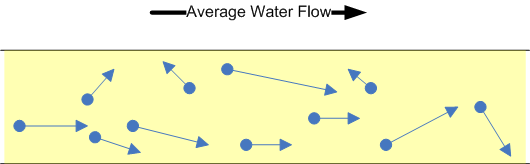
\includegraphics[width=80mm]{.//figures/water.png}
\caption{Microscopic View of Water Flow in a Pipe}
\vskip -6pt
\end{figure}

\subsection{Water Flow Rate Estimation using Vibration Sensors}
To formulate the model of NAWMS, we start with the microscopic view of water flow in a pipe given in [], build up some optimization problems depending on pipe topologies, which minimize performance metric of the system, namely the sum of estimation error.  

\subsubsection{Theory of Operation}
This section describes how vibration on a pipe can be related to water flow rate in a pipe. Looking at water flow in a pipe in a microscopic way, there are many molecules flow toward the flow direction in average. Each molecule has its own velocity as shown in the figure 2. While water is flowing toward its flow direction, many molecules hit the pipe. According to the first law of thermodynamics, some of the kinetic energy is converted to heat as the turbulent eddies dissipate, but most is converted into potential energy in the form of pressure [Pittard 2003]. Evans et. al.p[  showed that the variance of vibration is proportional to the average flow rate in a pipe. The following is a brief excerpt from [Evans] that illustrate the mathematical model of this concept. 

The local velocity at a point can be regarded as superposition of an average velocity and instantaneous fluctuating velocity. The fluid velocities can be decomposed in time averaged velocities and fluctuation velocities. Let define  $u$ be the velocity parallel to the pipe axis and $v$ be the velocity perpendicular to the pipe axis. The instantaneous velocities $u,v$, can be written as a sum of the average velocities $\bar{u},\bar{v}$ and the fluctuation velocities $u',v'$. 
\begin{equation}
\begin{array}{l}
u=\bar{u}+u' \\
v=\bar{v}+v'=v'
\end{array}
\end{equation}
Since there is no net flow in the perpendicular direction to the pipe axis, the time averaged velocity $\bar{v}$is zero. 
Prashun[] showed that the time average of the product of the velocity fluctuation is less than zero. 
\begin{equation}
\overline{u'v'} < 0
\end{equation}
Prashun[] also demonstrated that for a circular conduit of radius $r$, the shear stress $\tau$ at the wall can be related to the pressure $p$ as follows.  
\begin{equation}
\begin{array}{l}
\tau=-\frac{r}{2}\frac{dp}{dx}\\\\
\frac{dp}{dx}=p'=-\frac{2\tau}{r}
\end{array}
\end{equation}
From the Navier-Stokes equations, Prashun[] also demonstrated that for turbulent flow, the turbulent shear stress can be expressed as
\begin{equation}
\tau=-\rho\overline{u'v'}
\end{equation}
Equations [][][] yield that the pressure fluctuation is proportional to the fluctuation of the fluid velocity. 
\begin{equation}
p' \propto \overline{u'v'}
\end{equation}
In addition, it can be shown that the pipe vibration is proportional to the pressure fluctuations in the fluid. First, the fluid filled pipe system can be depicted as a one-dimensional model of a beam. It is well known from structural mechanics that the rate of change of the moment along a beam is equal to the shear and the rate of change of shear, $dV/dx$, along the length of the beam is equal to the pressure fluctuations, $p'(x)$, per unit length as
\begin{equation}
\frac{d^{2}M}{dx^{2}}=\frac{dV}{dx}=p'(x)
\end{equation}

When a beam is subjected to bending, one side of the beam is in tension while the other side is in compression. Differentiating the Flexture Equation () twice with respect to x, then using the relationship for p� gives

\begin{equation}
\begin{array}{l}
M=EI\frac{d^{2}y}{dx^{2}} \\\\ 
\frac{d^{2}M}{dx^{2}}=EI\frac{d^{4}y}{dx^{4}}=p'(x)
\end{array}
\end{equation}

To relate the pressure fluctuations to the pipe acceleration, consider the differential equation of motion for transverse vibration of a beam as given by Seto[]
\begin{equation}
\frac{\partial ^{2}y}{\partial t^{2}}=-\frac{EIg}{A\gamma}\frac{\partial ^{4}y}{\partial x^{4}}
\end{equation}
where

$A$ : cross sectional area of the beam

$\gamma$ : specific weight of the beam

$g$ : gravity

$EI$ : flexural rigidity

Since $A$, $g$, and $\gamma$ are constant, equation () can be rewritten for convenience

\begin{equation}
\frac{\partial ^{2}y}{\partial t^{2}}=-CEI\frac{\partial ^{4}y}{\partial x^{4}}=-Cp'(x)
\end{equation}

where $C=\frac{g}{A\gamma}$

This indicates that the acceleration of the pipe is proportional to the pressure fluctuations in the fluid. The basic theory of operation will be based on the relationship between the standard deviation of the pipe vibrations and the mean flow rate of the fluid in the pipe. Blake[] stated that the generation of vibrations by fluid motion involves the reactions of fluids and solids to stresses imposed by time-varying flow. For dynamically similar flows, the radio of the flow fluctuations to the average flow is constant. Bird et. al.[] showed that this relationship by noting that the oscillatory term is the time average of the absolute magnitude of the oscillation, given by  where  . They defined this as �intensity of turbulence,� which is a measure of the magnitude of the turbulent disturbance, and is given by $\frac{\sqrt{\bar{m}}}{\bar{u}}=$ intensity of turbulence

From the definition of turbulent flow, the intensity of turbulence expression can be rearranged as
\begin{equation}
\frac{\bar{m}}{\bar{u}^{2}}=\frac{\frac{1}{N}\sum_{i=1}^{N}\left[u_{i}(t)-\bar{u}\right]^{2}}{\bar{u}^{2}}
\end{equation}

Multiplying both side by the number of points N and $\bar{u^{2}}$ and dividing by N-1, we get
\begin{equation}
\frac{1}{N-1}\sum_{i=1}^{N}\left[u_{i}(t)-\bar{u}\right]^{2}=\frac{NC}{N-1}\bar{u}^{2}=K\bar{u}^{2}
\end{equation}

This shows the flow fluctuations are proportional to the pressure fluctuations and the pressure fluctuations are proportional to the pipe vibration, it also follows that the standard deviation of the pipe vibrations is proportional to the average flow rate.
This result doesn�t necessarily show that the water flow rate in a pipe is linearly proportional to the vibration on the pipe. Instead they have a non-linear but proportional relation due to non-linear characteristics of vibration sensors, pipe structure, turbulence, etc. Experimental result in section ?? shows this relationship.

\subsubsection{ Vibration to Flow Rate Model}
\begin{figure}
\centering
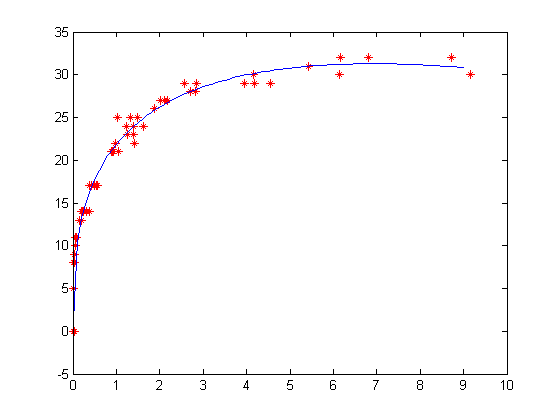
\includegraphics[width=80mm]{.//figures/copper.png}
\caption{Copper Pipe Vibration to Water Flow Rate}
\vskip -6pt
\end{figure}

Although the concept given in section 3.1.1 will be shown in section 4 through elaborate experimental  results, this section briefly introduce the vibration to the flow rate model to formulate a large scale water flow rate monitoring system using less intrusive vibration sensors. To see the relationship between vibration and water flow rate, we measured vibration on a pipe and water flow rate in the pipe while changing water flow rate by changing faucet   valve position. Figure ?? illustrate that water we may fit the curves and the fitted curve equations are as follows,
\begin{equation}
f(t)=\alpha \sqrt[3]{v(t)}+\beta \sqrt{v(t)}+\gamma v(t) + \delta
\end{equation}
where

$f(t)$ : water flow rate

$v(t)$ : vibration

Section 4.? will describe this model gives less error thus is the best and simple form, we took the model for vibration to flow rate relationship to construct the large scale water flow rate monitoring system. 

\subsection{Simple Pipe Structure}
\begin{figure}
\centering
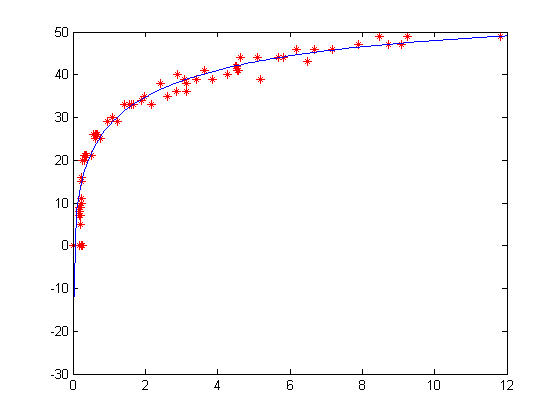
\includegraphics[width=80mm]{.//figures/pvc.png}
\caption{PVC Pipe Vibration to Water Flow Rate}
\vskip -6pt
\end{figure}


In this section, we formulate the large scale water flow rate monitoring system that consists of one main water meter, many vibration sensors on pipes, and an aggregation unit. Using the information from the main water meter that is more accurate but lacks spatially finer grained information, the system calibrates parameters (alpha, beta, gamma and delta) of every vibration sensors while solving an optimization problem. This problem can be generalized for more general pipe topologies shown in figure ?? and we will discuss this in the next section. Firstly, consider a simple  pipe topology where one main pipe is equipped with he main water meter and N pipe branches where we put vibration sensors. The main water meter gives us its real-time water flow in the main pipe and let define $M(t)$ as water flow rate of the main pipe. Let define the water flow rate of each branches as $f_{i}(t)$ where $i$ is pipe index number. Since all branches are connected to the main pipe, we can immediately get eq() because the total water flow rate is the sum of all the flow rate in every pipe branches.

\begin{equation}
M(t) = \sum _{i=1} ^{N} f_{i}{(t)}
\end{equation}
where

$N$: Total number of pipes

From section 2, we approximate mapping from variance of vibration on a pipe to actual water flow rate in the pipe as follows,[model validation needed]

\begin{equation}
f_{i}(t)=\alpha_{i} \sqrt[3]{v_{i}(t)}+\beta_{i} \sqrt{v_{i}(t)}+\gamma_{i} v_{i}(t) + \delta_{i}
\end{equation}

According the relationship shown in section 3.1.1, it has to be a linear mapping from the variance of vibration to the flow rate. Due to sensor and pipe saturation and unmodeled parameters as mentioned earlier, we put additional terms to capture these. 

In order to estimate $\alpha_{i}, \beta_{i}, \gamma_{i}$, and $\delta_{i}$ one can calibrate each sensor at a time using a vibration sensor and water flow meter pair, however it requires manual effort that increases installation cost. We want to avoid this to reduce installation by introducing an optimization problem that yields all the parameters.

Assume every sensor samples every $\Delta t$ and every sensor is synchronized. Consider equation () and we get $M(\Delta kt) = \sum_{i=1}^{N} f_{i}(\Delta kt)$

After getting M samples, we get $\sum_{k=1}^{M}M(\Delta kt) = \sum_{k=1}^{M}\sum_{i=1}^{N} f_{i}(\Delta kt)$ 

Since we know this equality always holds unless there is water leakage, we can formulate this as an optimization problem as follows
\begin{equation}
\begin{array}{ccc}
min &&\left|\left|\sum_{k=1}^{M}M(\Delta tk) - \sum_{k=1}^{M}\sum_{i=1}^{N} f_{i}(\Delta tk)\right|\right|_{1}\\\\
subject & to & \\\\
&&
0 \leq f_{i}(\Delta tk) \leq f_{i},max 
\end{array} 
\end{equation}
where

$f_{i}(\Delta tk)=\alpha_{i}\sqrt[3]{v_{i}(\Delta tk)}+\beta_{i}\sqrt{v_{i}(\Delta tk)}+\gamma_{i}v_{i}(\Delta tk)+\delta_{i} $

$\Delta t$ : Sampling Time 

$M$ : Number of Samples

$N$ : Number of Pipes
\\


Solving this optimization problem yields all the necessary parameters if it gives the global optimum and is only one point. This equation also implies that for the calibration no human intervention is needed as the optimization and sampling can be automated. Note that, this optimization problem consists only of linear constraints and its objective function can be also formulated as a linear objective function[]. Therefore, any available LP solver can solve this problem very efficiently and guarantees global optimum.

\subsection{General Pipe Structure}
\begin{figure}
\centering
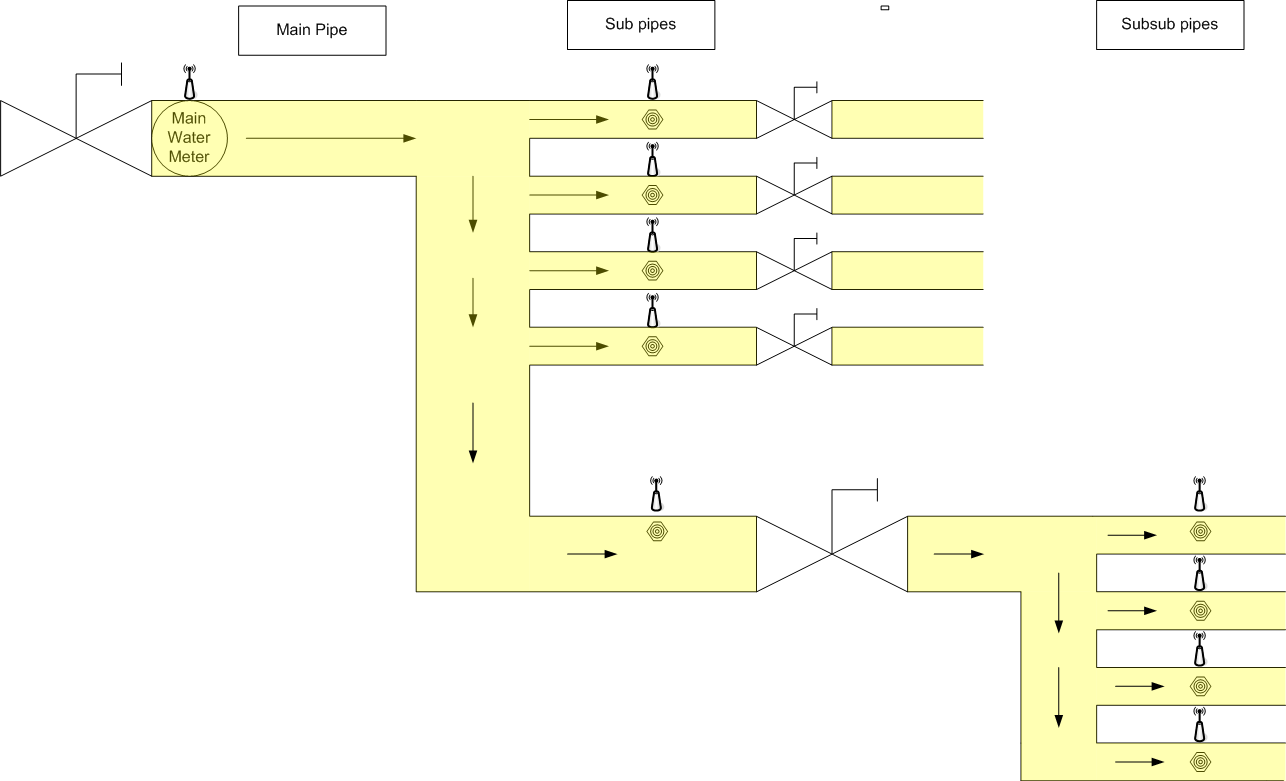
\includegraphics[width=80mm]{.//figures/pipes2.png}
\caption{Complex Pipe Topology}
\vskip -6pt
\end{figure}

Since this optimization problem minimizes the error; (Total Water Flow Rate - Sum of Water Flow Rate of every pipe branches), it guarantees minimum error in its estimation. However section 3.2 only considers one simple pipe topology, in this section we consider a more general topology of pipe structure and show that the problem can be decomposed depending on their topology. This might have more than one optimization problem but can be solved very efficiently in known polynomial time. Thus, we describes how to decompose a more complex topology of the pipes but rest of the paper focuses on the first problem() as each of optimization problem can be dealt with separately.  
Consider a pipe structure in figure ??, assuming there is no water leakage, the total flow rate must be the sum of water flow rate of sub pipes. Similarly the flow rate of each sub pipe must be the sum of flow rate of its sub-sub pipes. Therefore we have K equalities that need to hold to satisfy the law of mass conservation. 
Let define the water flow rate in a pipe as 
$f_{i,j}(t)$ where $i$ is sub pipe index and $j$ is sub-sub pipe index

Due to the law of mass conservation, these two equations must hold unless there's water leakage in a pipe
\begin{equation}
\begin{array}{l}
f_{i}(t) = \sum_{j=1}^{J}f_{i,j}(t)\\
 M(t) = \sum_{i=1}^{N}f_{i}(t)
\end{array}
\end{equation}
\\

From the equations () and (), we can immediately get the following which is a slight modification of equation (). 

\begin{equation}
\begin{array}{ccc}
min &&\left|\left|\sum_{k=1}^{M}M(\Delta tk) - \sum_{k=1}^{M}\sum_{i=1}^{N} f_{i}(\Delta tk)\right|\right|_{1}\\\\
subject & to & \\\\
&&
0 \leq f_{i}(\Delta tk) \leq f_{i},max \\\\
&& f_{i}(\Delta kt) = \sum_{j=1}^{J_{i}}f_{i,j}(\Delta kt)
\end{array} 
\end{equation} 
where

$f_{i}(\Delta tk)=\alpha_{i}\sqrt[3]{v_{i}(\Delta tk)}+\beta_{i}\sqrt{v_{i}(\Delta tk)}+\gamma_{i}v_{i}(\Delta tk)+\delta_{i} $

$\Delta t$ : Sampling Time

$M$ : Number of Samples

$N$ : Number of Pipes 

$J_{i}$ : Number of sub-pipe branches of i-th sub-pipe of the main pipe
\\


Similarly, this concept can be generalized as the main pipe water flow rate is the sum of its sub pipe branches, a sub pipe branch flow rate is the sum of its sub-sub pipe branches and so forth. 
Therefore, depending on users� need, one can always make these equalities to formulate similar problem forms. For example, if they are interested in the water flow rate to the bathroom rather than each of bathroom sink, toilet bin, and  shower booth, they want to omit individual pipe, instead they want to monitor a sub pipe that has each of branches. 
 
 \subsection{Account for Vibration Propagation}

 \begin{figure}
\centering
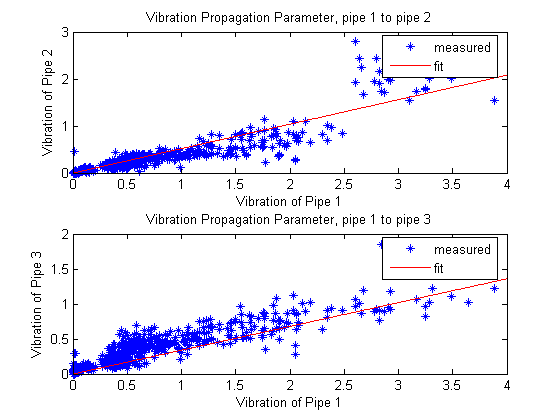
\includegraphics[width=80mm]{.//figures/P123.png}
\caption{Vibration Propagation from Pipe 1 to Pipe 2 and Pipe 3}
\vskip -6pt
\end{figure}

 \begin{figure}
\centering
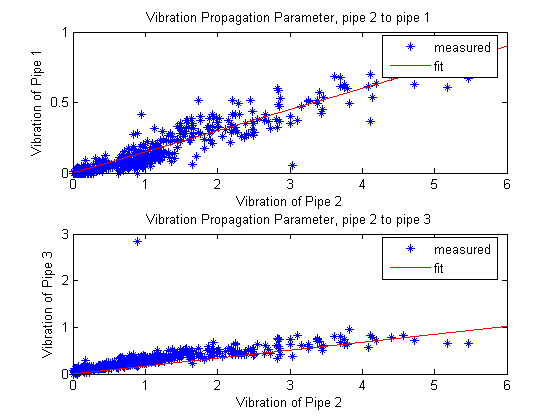
\includegraphics[width=80mm]{.//figures/P213.png}
\caption{Vibration Propagation from Pipe 2 to Pipe 1 and Pipe 3}
\vskip -6pt
\end{figure}

 If we consider a pipe structure in figures ?? and ??, we didn�t take vibration propagation among pipes into account. However, pipes are physically connected and metal and PVC pipes are pretty good material that transfer vibration among themselves. Therefore, the model needs to consider vibration propagation among pipes and compensate this effect to achieve better precision. 
In general, the vibration propagation may not be linear because pipe topology could be very complex, connection among pipes may consist of hybrid material, different types of mechanical structure have different resonance frequency, etc. Since the water flow induced vibration if relatively small, we want to assume that the vibration propagation is linear and show this through our experiment in section 4.??. 
Consider there is vibration only on pipe j and let first define propagation parameter from pipe i to pipe j as
 
 \begin{equation}
 v_{m,i}(t) = p_{i,j}v_{j}(t)
 \end{equation}
 
 where
 
 $v_{m,i}(t)$ : measured vibration on pipe i
 
 $p_{i,j}$ : Vibration Propagation Constant from pipe j to pipe i
 
 $v_{j}(t$ : Water Flow induced Vibration on pipe j
\\

Since we see this vibration is linear, the measured vibration on the pipe i is the superposition of all possible vibrations from pipe 1 to N as follows

\begin{equation}
v_{m,i}(t) = \sum_{j=1}^{N}p_{i,j}v_{j}(t)
\end{equation}
where

$v_{m,i}(t)$ : Measured Vibration on pipe i
$p_{i,j}$ : Vibration Propagation Coefficient
$v_{j}(t)$ : : Water Flow induced Vibration on pipe j

Note also that, 

$p_{i,j} = 1$  if $i=j$

$0 \leq p_{i,j} \leq 1$ otherwise

Because the pipe architecture is passive, its propagation coefficient cannot exceed 1 and cannot be less than zero.  Once we model this, we can immediately get the following optimization problem by modifying the problem () in section 3. 

\begin{equation}
\begin{array}{ccc}
min &&\left|\left|\sum_{k=1}^{M}M(\Delta tk) - \sum_{k=1}^{M}\sum_{i=1}^{N} f_{i}(\Delta tk)\right|\right|_{1}\\\\
subject & to & \\\\
&&
0 \leq f_{i}(\Delta tk) \leq f_{i},max \\\\
&&v_{m,i}(t) = \sum_{j=1}^{N}p_{i,j}v_{j}(t) \\\\
\end{array} 
\end{equation}

where 

$\Delta t$ : Sampling Time

$M$ : Number of Samples

$N$ : Number of Pipes
\\

Because of propagation effect that adds one posynomial equality constraint, this problem becomes a nonlinear and non-convex optimization problem that is extremely hard to solve. However, we explore two methods of reformulating the problem either as a generalized geometric programming  problem by relaxing and restricting constraints with reasonably tight bound while conserving physical meaning of the problem or as a two phase linear programming problem by decomposing the optimization problem into two problems. It is well known that both geometric programming and linear programming problems can be solved in polynomial time. The following two subsections describe the GP modeling of the problem and the two phase LP modeling and show that one can solve these.
Depending on the system performance and its characteristics, the system can select either one of both optimization problems to achieve its desired accuracy.

\subsection{ Geometric Programming Modeling}
The posynomial equality constraint prevents us to solve the optimization problem as a geometric programming. In addition, the objective function is not a standard geometric programming form. 
\begin{equation}
v_{m,i}(t) = \sum_{j=1}^{N}p_{i,j}v_{j}(t)
\end{equation}

Therefore, we need to reformulate this optimization problem because this problem is in general NP-hard. In this section we describe a derivation of this non-convex optimization to a convex optimization problem with careful modification while maintaining physical meaning of the optimization problem. 
First, we introduce a slack variable s and the problem can be equivalently reformulated as follows,

\begin{equation}
\begin{array}{ccc}
min && s \\\\
subject & to & \\\\
&& -s \leq \sum_{k=1}^{M}\sum_{i=1}^{N} f_{i}(\Delta tk) - \sum_{k=1}^{M}M(\Delta tk)  \leq s\\\\
&&
0 \leq f_{i}(\Delta tk) \leq f_{i},max \\\\
&&v_{m,i}(t) = \sum_{j=1}^{N}p_{i,j}v_{j}(t) 
\end{array} 
\end{equation}

By restricting the original objective function as follows,
\begin{equation}
0 \leq \sum_{k=1}^{M}\sum_{i=1}^{N} f_{i}(\Delta tk) - \sum_{k=1}^{M}M(\Delta tk)  \leq s
\end{equation}

Therefore, we can obtain the following,
\begin{equation}
\begin{array}{ccc}
min && s \\\\
subject & to & \\\\
&& 0 \leq \sum_{k=1}^{M}\sum_{i=1}^{N} f_{i}(\Delta tk) - \sum_{k=1}^{M}M(\Delta tk)  \leq s\\\\
&&
0 \leq f_{i}(\Delta tk) \leq f_{i},max \\\\
&&v_{m,i}(t) = \sum_{j=1}^{N}p_{i,j}v_{j}(t)
\end{array} 
\end{equation}

Now, according to [GP COMM], by relaxing the posynomial equality constraint as an inequality with reasonable tightness, one can reformulate the constraint as a standard geometric programming form. The following relaxation is reasonable as the measured variance of vibration on a pipe is not only the superposition of all the propagated vibration but also from the external vibration source. 

\begin{equation}
\sum_{j=1}^{N}p_{i,j}v_{j}(t) \leq v_{m,i}(t)
 \end{equation}
 As a consequence, we can obtain the following optimization problem, 
 
 \begin{equation}
 \begin{array}{ccc}
min && s \\\\
subject & to & \\\\
&& \sum_{k=1}^{M}\sum_{i=1}^{N} f_{i}(\Delta tk)  \leq s + \sum_{k=1}^{M}M(\Delta tk)\\\\
&&
0 \leq f_{i}(\Delta tk) \leq f_{i},max \\\\
&&  \sum_{j=1}^{N}p_{i,j}v_{j}(t) \leq v_{m,i}(t)
\end{array} 
\end{equation}

where

$f_{i}(\Delta tk)=\alpha_{i}\sqrt[3]{v_{i}(\Delta tk)}+\beta_{i}\sqrt{v_{i}(\Delta tk)}+\gamma_{i}v_{i}(\Delta tk)+\delta_{i} $
\\

According to [GP TUTORIAL] in section 7.3, it is a mixed linear geometric programing, as equation() is a posynomial because eq() is posynomial.

equation () is posynomial as all the alphas, betas, gammas and deltas are positive, and vibration is always positive.
and the sum of posynomials is also a posynomial and because variance is positive by its nature. 
Therefore, one can solve this problem very efficiently (polynomial time) and guarantees the global optimum as it turns out to be a convex programming problem[]. However, this might render a poor solution as we relaxed the constraint although it is reasonable relaxation. Therefore, we also want to introduce two phase Linear Programming program in case it render a poor solution so that the system can select one

\subsection{ Two phase Linear Programming Modeling}
While section 3.5 gives us a convex optimization problem that gives a set of parameters needed for estimating water flow rate in a pipe, one can further reduce its computational complexity if we derive this as an approximate Linear Programming problem. Although propagation parameters are unknown, since pipe topology is static and not changing over time, one can measure propagation parameters in its initial stage. Then ? are constant and can be estimated.
Once propagation parameters are estimated, ? can be obtained thus its posynomial equality term becomes a linear equation. Therefore, the problem can be decomposed into two problems; a) propagation parameter estimation problem and b) water flow rate function coefficient estimation problem. 
\subsubsection{Vibration Propagation Parameter Estimation}
As it is possible to have situation where only one pipe is on at a time during a long period of time, the system can measure vibration on every pipe and water flow happens on a single pipe j. The measured vibration on the pipe j and the water flow induced vibration on the pipe j is the same, thus we get
$v_{m,j}=v_{j}$

Therefore, measured vibration on each of pipe can be expressed as follows

$v_{m,i} = p_{i,j}v_{m,j}$

It is also obvious that 

$p_{i,j}=1$ if $i=j$

$p_{i,j} = \frac{v_{m,i}}{v_{m,j}}$ otherwise

If the system is ideal, the measurement is perfect, and the system model is flawless, then the propagation parameter estimation is trivial as shown above. However, as most of parameter estimation problem relies on some estimation procedure such as least square estimation, 1-norm minimization approach, or infinity-norm minimization approach due to measurement noise, we also need to formulate this as an parameter estimation problem because the system model, sensors and environment are not ideal thus have measurement noise and unmodeled uncertainties. We want to set the problem as a 1-norm minimization problem with some linear inequality constraints as it is less sensitive to the significant outlier than least square problems and this is mainly because cheap sensors and many wireless sensor nodes often suffer from significant outliers and faulty sensor reading[][][]. We can solve this problem using standard LP solvers and also can easily handle linear inequality constraints.

Let define $l$ be a index of sample and $L$ be the total number of samples.
\begin{equation}
\begin{array}{ccc}
min &&\left|\left| \sum_{l=1}^{L}v_{m,i}(l) - \sum_{l=1}^{L}p_{i,j}v_{m,j}(l)\right|\right|_{1}\\\\
subject & to & \\\\
  && 0 \leq p_{i,j} \leq 1 \\
&&p_{i,i} = 1
\end{array} 
\end{equation}


\subsubsection{ Vibration Parameter Estimation}
After getting vibration propagation parameters, the problem simply becomes a typical linear programming problem as a matrix P is invertible. Therefore, we get
\begin{equation}
\begin{array}{ccc}
min &&\left|\left|\sum_{k=1}^{M}M(\Delta tk) - \sum_{k=1}^{M}\sum_{i=1}^{N} f_{i}(\Delta tk)\right|\right|_{1}\\\\
subject & to & \\\\
&&
0 \leq f_{i}(\Delta tk) \leq f_{i},max \\\\
&&V(t) = P^{-1}V_{m}(t) \\\\
where && \\\\
&& P = [ p_{i,j} ] \\
&& V(t) = [v_{i}(t)] \in R_{+}^{N} \\
&& V_{m}(t) = [v_{m,i}(t)] \in R_{+}^{N}\\

&&\Delta t : Sampling Time \\\\
&&M : Number of Samples\\
&&N : Number of Pipes 

\end{array} 
\end{equation}

So, this form is again a linear programming problem thus one can solve this problem and get parameters. 

\subsection{ Correction Mechanism}
After getting all the necessary parameters by solving the optimization problems given in section ??, the system can estimate the water flow rate of each pipe based on vibration. However, unpredicted turbulence in a pipe, external vibration, etc. can make the estimate less accurate. To compensate these, the system also takes advantage of the water flow rate from the main pipe. 
Considering the water flow rate is the same as the sum of the water flow rate of every branch of the main pipe. We normalize the water flow rate estimate as follows

\begin{equation}
f_{i}(t) = \frac{\hat{f_{i}}(t)M(t)}{\sum_{i=1}^{N}\hat{f_{i}}(t)}
\end{equation}

This normalization may add small error to the water flow rate estimate. It guarantees, however, that the sum of the water flow rate estimate as well as the sum of the accumulated water usage estimate is the same as the true water flow rate and accumulated water usage.


\section{ NAWMS Architecture}
  \label{sec:architecture}
To make the system mass deployable and to reduce cost, NAWMS exploits many available options. Especially, it extensively uses commercially available devices to infer water flow rate in a pipe in a nonintrusive way while leveraging pre-existing information from the infrastructure, namely the main water meters for billing purpose. 
The main three components of the system consist of : 
 Snooping of Existing Infrastructure; The main water meter provides accurate water flow rate as it is meant to be for billing purpose. It, however, lacks spatial granularity as it only needs to monitor water flow rate to the entire household. Spatially finer granularity is not necessary for the main water meter. 
 Wireless Sensor Nodes; it inherently has many types of sensing modalities. The system uses accelerometer to measure water flow rate relying on mechanical characteristics of water flow and pipe structure.
 Open Source Optimization Toolbox; calibration requires much time and human intervention. This paper propose several types of optimization problems that enable the system to calibrate its parameters and coefficients automatically. 

\subsection{ Snooping of Existing Infrastructure }
  \label{subsec:snooping}
Available technologies for resource monitoring either provide information at coarse spatial granularity, like the water meters for an apartment. The problem is that they miss to show the consumption at a per individual level. 
However, they provide accurate sensor reading that helps calibrate sensors that monitor physically connected sensors as they are less precise as shown in section 3, but monitor partial information of the main water meter. As we have shown in section (), we make use of this relatively accurate information to maximize monitoring accuracy. In other words, NAWMS aims to aggregate both types of information, M(t) ad v(t), to hit the balance among these conflicting criteria. Since most households already have measurement units, e.g. water meters, NAWMS snoops the information from the main water meter.  
To get real-time information from the water meter, some technology can be used\cite{C700pulser}, \cite{AWWA2005}. \cite{C700pulser} is one way to get an accurate water flow rate of the main water pipe in a house as it provides pulse train depending on the actual water flow rate in a pipe. Most of wireless sensor nodes can get this information and provides real-time water flow rate to the place where it is needed. In addition, Automatic Meter Reading Association\cite{AMRA} and American Water Works Association \cite{AWWA2005} are building systems that can provide near real-time meter information for billing purpose and we believe that $M(t)$ shown in section ?? can be readily available in the near future. 

\subsection{ Nonintrusive Water Flow Rate using WSNs}
  \label{subsec:vibrationsensors}
Intuition tells us that vibration of a pipe can be a metric to estimate water flow rate in a pipe. The sophisticated theory of operation is give in section ??. This section describes its hardware set-up to monitor water flow induced vibration in a pipe. 
We used MicaZs with MTS310\cite{Xbow} data acquisition boards running SOS operating system\cite{sos05mobisys} to measure vibration on a pipe. The MTS310 sensor board includes several sensors such as microphone, accelerometer, magnetometer and photo-resistive light sensor. We only used one analog device ADXL202 accelerometer that is capable of measuring $+-2g$ range of acceleration. To achieve better accuracy, one can use more sensitive vibration sensors. Since the problems ()() constrain the maximum flow rate of each pipe, the external vibration will be disregarded. (good part!). To reduce development cost, we took this as it achieves reasonable accuracy as the overall precision is benign and is for human reading purpose for now. 
A static SOS application samples acceleration 100Hz, after getting 50 samples, it locally calculates sample variance of acceleration and we consider this as measure of vibration\cite{EvansFlowMeasurement}, \cite{Bird1960}, \cite{Fogarty2006}, \cite{Pittard2003}. As it processes the data locally and send the vibration information back to the aggregation every one second, its communication cost is low. It is also obvious the from the equation() the measure of vibration of this case is the sample variance of acceleration perpendicular to the pipe axis.

\subsection{Optimization Toolbox}
  \label{subsec:optimizationtool}

To solve the optimization problems given in section ??, we used CVX toolbox \cite{CVXOPT}, \cite{BoydTutorial2005} that is an open source convex optimization tool and has python, c, and Matlab interfaces. Its efficiency and reliability is known to be good and it can solve most of convex optimization problem in polynomial time while guaranteeing robust solution that is also a global optimum. More complicated tool also can be used \cite{MOSEK} since they provide student license for free, but our optimization is well fit to the CVX thus we just used that one. 



\section{Evaluation}
This section elaborates experimental results that support the models and formulations shown in section 3. In section 5.1, we describe the evaluation setting including hardware and software architecture, and prototype pipe system. Section 5.2 describes measured vibration on a pipe and its mapping to the actual water flow rate in the pipe. It evaluates its performance against the ground truth obtained from the water flow meter. Section 5.3 shows the end result of the system. 

\subsection{ Deployment Setting System Architecture}
As shown in Figure ??, the design of the NAWMS system consists of tiered sensor system and a custom pipe system. The pipe system is made of one main pipe and three branches; one branch is ?? copper pipe, one is ?? size PVC pipe and the other one is ?? size PVC pipe. The main pipe is equipped with an commercial water flow meter that generates pulse train whose pulse speed is proportional to the actual flow rate. Each branch is equipped with an acceleration sensor that is a part of MTS310 sensor board. MicaZ is used to collect and process sensor data and is running SOS operating system[]. The vibration mote samples acceleration perpendicular to the pipe surface. To get vibration measure, it sample 50 data points at 100Hz every one second, then calculate sample variance that is the measure of vibration. The main water meter mote counts the number of pulses per a second and sends it back to the laptop. The laptop aggregates vibration on each pipe and water flow rate in the main pipe. It also solves the optimization problem after it receives sufficient data set using CVX[]. After solving the optimization problems, it renders water flow rate in each of the branches.

\subsection{ Evaluation of Water Flow Rate Estimate}
This subsection elaborates step-by-step validation of the models shown in section ??. First, section 5.2.1 validates equation () by comparing several models. To show its performance, we also give the evaluation against the ground truth. Section 5.2.2 shows propagation model validation through some experimental result. Section 5.2.3 shows its data after solving the optimization problem and shows how it looks like.

\subsubsection{ Vibration to Water Flow Rate Model Validation }
From the equation (), one may expect the vibration to the water flow rate relation is linear. However, unmodelled parameters and sensor characteristics make the relationship nonlinear as shown in the figure. Getting a realistic model that well fits to the real relation is of importance to minimize the estimation error. Many model can be derived from the observation but decision relies on our heuristics. Most popular model for the curve fitting is polynomial curve fitting, but figure ?? shows saturation which is similar to square root curve or log curve. For comparison, we picked a 4th order polynomial fitting and 3rd root fitting shown in equation ??. We discarded log model to make the optimization problem solvable. 

\subsubsection{ Vibration Propagation among pipes }
As mentioned in section, we also validated that vibration propagation happens among pipes and can be approximated with the model given in equation (). 
To see the propagation from pipe 1 to pipe 2 and 3, we only turned on each of pipes at a time and plotted vibration on pipe i versus vibration on pipe j. Figures ??,??,?? and ?? show that the propagation can be approximated with a multiplicative coefficient. It comes with big variation that results in the water flow rate estimate error. (how do you).

\subsubsection{ Data Representation }
Figures ?? and ?? give an example of water flow rate estimate of two pipes. Two metrics are considered because instant water flow rate estimate and accumulated water usage are both important. In figure ??, lower plot shows the water flow rate in the main pipe from the water flow meter. In the upper plot, blue line shows the sum of both pipies� water flow rate estimate, red line shows water flow rate estimate of pipe 1, and magenta line shows water flow rate estimate of pipe 2. Since we aim to minimize the sum of water flow rate estimate error, we can see in the figure that the sum of water flow rate estimate and the true water flow rate is the same as the system normalized the estimate based on the main water flow meter.
Similarly, figure ?? shows the accumulated water usage estimate from the figure. And two blue lines in the upper and lower figures are the same because of equation()



\section{Conclusion}
We introduced less intrusive and auto calibrated individual pipe level water monitoring system that provides spatially finer grained water usage profile that helps people conserve water resource in a house hold. The solutions of the optimization problems yield calibration parameters and vibration propagation parameters that minimize the sum of estimation error. Our experimental results showed that the vibration based water flow rate estimation is feasible as it renders reasonably small error. 
We also envision that this information helps classify water related activities similar to [Fogarty] and further classification accuracy. It may also be used for detecting water leakage by determining if there�s excessive water flow happens on a pipe than the normal operation along a similar line of [Structure Monitoring]. 

\section{ Future work}
The limitation of the current system is that it requires us to put many sensors on every pipe of interest, that may increase hardware cost as the pipe system becomes complex and has many pipes. We will explore ways of estimating water flow rate using less amount of sensors considering pipe topology. 
With slight modification, we envision the proposed frame work can also be used for electrical energy consumption as it consists of the main power meter for billing purpose and some less intrusive sensors that need to be calibrated are available [leland]. 
In terms of applications, activity classification can be very interesting as water usage often requires human presence and the water related activities result in water consumption similar to [], but can provide more meaningful information for users in terms of natural resource consumption profile associated with activities thus help people improve their resource efficiency. 
% end the environment with {table*}, NOTE not {table}!

\bibliography{SpotLight}

\end{document}
